%%%% Paramétrage du TD %%%%
\def\xxactivite{\ifcolle Colle \else TD 2 \fi  \ifprof -- Corrigé \else \fi} % \normalsize \vspace{-.4cm}
\def\xxauteur{\textsl{Xavier Pessoles}}

\def\xxnumchapitre{Chapitre 3 \vspace{.2cm}}
\def\xxchapitre{\hspace{.12cm} Méthodologie : détermination des équations de mouvement}
\def\xxpartie{Modéliser le comportement des systèmes mécaniques dans le but d'établir une loi de comportement ou de déterminer des actions mécaniques en utilisant le PFD}



\def\xxtitreexo{Dynamique du véhicule -- Véhicule à trois roues Clever\ifnormal $\star$ \else \fi \ifdifficile $\star\star$ \else \fi \iftdifficile $\star\star\star$ \else \fi }

\def\xxsourceexo{\hspace{.2cm} \footnotesize{Concours Banque PT -- SIA 2013}}


\def\xxcompetences{%
%\vspace{-.5cm}
\textsl{%
\textbf{Savoirs et compétences :}
\begin{itemize}[label=\ding{112},font=\color{ocre}] 
%\item \textit{Mod2.C16} : torseur cinétique
%\item \textit{Mod2.C17} : torseur dynamique
%\item \textit{Mod2.C17.SF1} : déterminer le torseur dynamique d’un solide, ou d’un ensemble de solides, par rapport à un autre solide
%\item \textit{Mod2.C15} : matrice d'inertie
\item \textit{Res1.C2} : principe fondamental de la dynamique
\item \textit{Res1.C1.SF1} : proposer une démarche permettant la détermination de la loi de mouvement
%\item \textit{Res1.C2.SF1} : proposer une méthode permettant la détermination d’une inconnue de liaison
\end{itemize}
}}
\def\xxfigures{
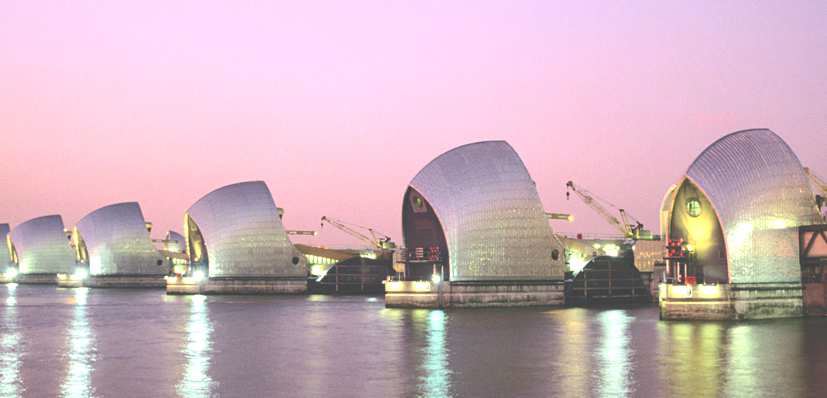
\includegraphics[width=.5\linewidth]{fig_00}
}%figues de la page de garde


\input{\repRel/Style/pagegarde_TD}
\setcounter{numques}{0}

\setlength{\columnseprule}{.1pt}

\pagestyle{fancy}
\thispagestyle{plain}

\ifprof
\vspace{4.8cm}
\else
\vspace{4.8cm}
\fi

\def\columnseprulecolor{\color{ocre}}
\setlength{\columnseprule}{0.4pt} 

%%%%%%%%%%%%%%%%%%%%%%%

\setcounter{exo}{0}

\ifprof
%\begin{multicols}{2}
\else
\begin{multicols}{2}
\fi




Le Clever%, présenté sur la \autoref{fig_01}, 
est un démonstrateur technologique développé par un tissu d'industriels européens.% — dont BMW, l'Institut Français du Pétrole (IFP) et de nombreux équipementiers — grâce au financement de l'Union Européenne. Clever est la contraction de Compact Low Emission VEhiclefor uRban tRansportation (véhicule compacte à faibles émissions pour le transport urbain) car, avec une consommation de seulement \SI{2,5}{L/100km}, il s'annonce très écologique. Les premiers prototypes ont vu le jour en 2006. Ce type de véhicule pourrait être un des prochains commercialisés par BMW si le prix de vente peut être ramené sous la barre des \SI{10000}{euros}.

%\begin{center}
%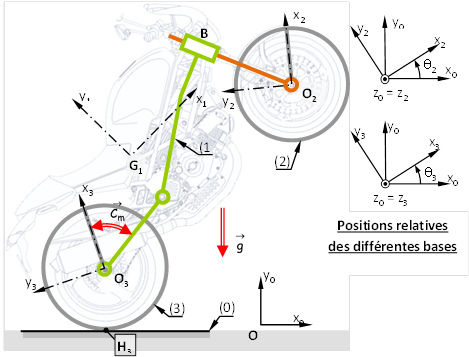
\includegraphics[width=0.5\linewidth]{fig_01}
%
%\textit{Véhicule à trois roues Clever \label{fig_01}}
%\end{center}

%La \autoref{fig_02} présente un diagramme partiel des interacteurs, issu de l'analyse fonctionnelle du besoin dans la phase d'utilisation normale (véhicule Clever utilisé pour se déplacer). Le Tableau \autoref{tab_01} décrit les fonctions de service correspondantes. À l'issue de l'analyse fonctionnelle technique, les solutions qui ont été retenues sont les suivantes : 
Il se présente comme un véhicule à trois roues pouvant embarquer deux personnes assises en tandem. Il adopte une architecture pendulaire, c'est-à-dire qu'il se penche dans les virages (cf. \autoref{fig_03}). Le déplacement du centre de gravité qui en résulte lui confère une grande stabilité malgré une faible largeur du véhicule (légèrement inférieure à \SI{1}{m}, contre 60 à \SI{75}{cm} pour une moto, et \SI{1,5}{m} pour une petite voiture). Cette étroitesse se veut une réponse aux problèmes d'encombrement dans les villes mais permet aussi une surface frontale moins importante que sur une voiture conventionnelle et donc des pertes aérodynamiques réduites. En outre, les sensations de conduite sont semblables à celle d'une moto mais avec un pilotage, à l'aide d'un volant, propre à un véhicule à 4 roues. Le moteur est un monocylindre à gaz naturel qui a été développé par l'IFP et dont les performances permettent d'atteindre une vitesse de pointe de $\SI{100}{km.h^{-1}}$ avec une accélération en phase avec les attentes pour un véhicule urbain.

\begin{center}
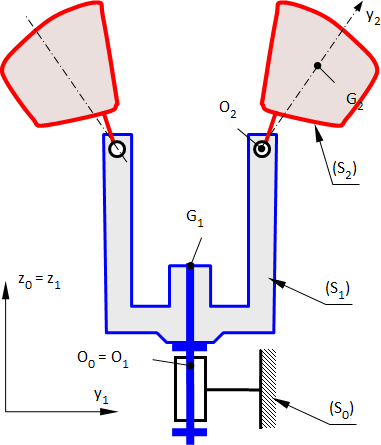
\includegraphics[width=\linewidth]{fig_02}

\textit{Diagramme partiel des interacteurs dans la phase d'utilisation normale}
\label{fig_02}
\end{center}

\begin{center}
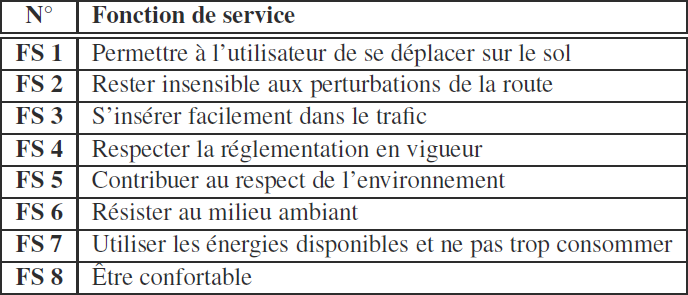
\includegraphics[width=\linewidth]{tab_01}

\textit{Caractérisation partielle des fonctions de service}
\label{tab_01}
\end{center}

Du point de vue de l'architecture cinématique (cf. \autoref{fig_03}), le groupe motopropulseur est placé à l'arrière. À l'avant, l'habitacle repose sur une roue de moto et pivote par rapport au bloc arrière autour d'une liaison pilotée angulairement par le biais de deux vérins hydrauliques. L'inclinaison est contrôlée par un ordinateur de bord en fonction de l'angle au volant et de la vitesse. Le Tableau \autoref{tab_02} regroupe les caractéristiques techniques annoncées par l'équipe de développement.

\begin{center}
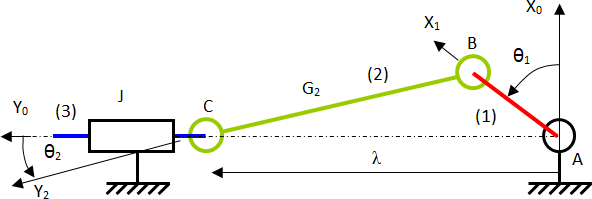
\includegraphics[width=0.8\linewidth]{fig_03}

\textit{Vue de la cinématique pendulaire}
\label{fig_03}
\end{center}

\begin{center}
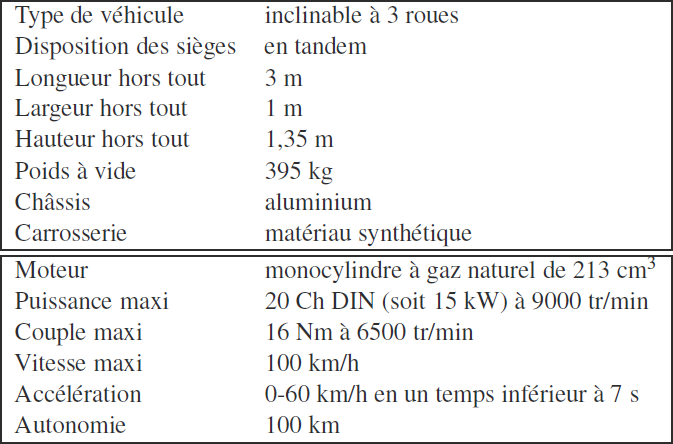
\includegraphics[width=\linewidth]{tab_02}

\textit{Caractéristiques techniques}
\label{tab_02}
\end{center}


%
%Travail demandé
%Ce sujet comporte 3 parties indépendantes, elles-mêmes constituées de nombreuses questions qui peuvent être traitées séparément :
%\begin{itemize}
%\item la Partie I (durée conseillée 1h30) se concentre sur la validation de la fonction technique « Modifier l'inclinaison de l'habitacle » ;
%\item la Partie II (durée conseillée 1h30) aborde la fonction technique « Transmettre la puissance mécanique » ;
%\item la Partie III (durée conseillée 1h30) concerne la fonction technique « Contrôler le mouvement de l'habitacle ».
%\end{itemize}
%Une lecture préalable du sujet complet est vivement conseillée (durée indicative 30 min).


%Applications numériques. -- Dans le domaine des Sciences Industrielles, le fait de savoir calculer et analyser les valeurs des grandeurs utiles au dimensionnement est aussi important que celui de savoir déterminer leurs expressions littérales. C'est pourquoi, une attention toute particulière sera accordée à la réalisation des applications numériques.
%
%Pour réaliser celles-ci sans l'usage d'une calculatrice, le candidat pourra faire des approximations de bon sens, qui conduiront éventuellement à une erreur relative de quelques pourcents sur le résultat final. Par exemple, dans le calcul suivant, qui fait intervenir l'accélération de la pesanteur $g = \SI{9,81}{m.s^{-2}}$, on pourra prendre :
% $$
% \dfrac{\pi^2}{2}\dfrac{100}{4}\left(5+3\times10^{-2}\right)g \simeq \dfrac{10}{2}\times 4 \times 5 \times 10 = \SI{1000}{m.s^{-2}}.
% $$

\section{Validation de la fonction technique « Modifier l'inclinaison de l'habitacle »}
\begin{obj}
Dans cette partie, on s'intéresse à la fonction technique « Modifier l'inclinaison de l'habitacle » qui a été proposée pour assurer les fonctions de service FS1 «Permettre à l'utilisateur de se déplacer sur le sol » et FS3 « S'insérer facilement dans le trafic » du Tableau \autoref{tab_01} donné en introduction. Ce choix doit en effet permettre de garantir la stabilité du Clever dans les virages tout en permettant une faible largeur du véhicule afin de s'insérer dans la circulation.
\end{obj}


On donne ci-dessous deux extraits du cahier des charges relatifs aux fonctions de service FS1 et FS3.

\begin{center}
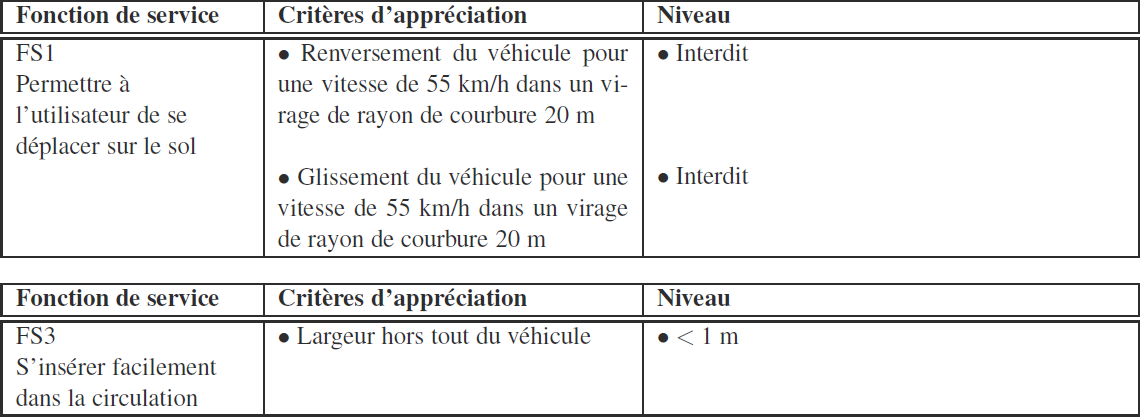
\includegraphics[width=\linewidth]{FS_01}
\end{center}


%\subsubsection*{Notations}
% Pour simplifier les notations dans ce sujet, le référentiel correspondant à un repère $\rep{i}$ est lui aussi désigné par $\rep{i}$. Les torseurs cinématique, cinétique et dynamique du mouvement du solide $j$ par rapport au solide $i$ (ou par rapport au référentiel $\rep{i}$ lié à celui-ci), exprimés en $A$, sont notés respectivement.
% 
%$$
%\torseurcin{V}{j}{i} = \torseurl{\vecto{j}{i}}{\vectv{A}{j}{i}}{A} 
%\quad
%\torseurci{j}{i} = \torseurl{\vectrc{j}{i}}{\vectmc{A}{j}{i}}{A} 
%\quad
%\torseurdyn{j}{i} = \torseurl{\vectrd{j}{i}}{\vectmd{A}{j}{i}}{A} 
%$$
%
%Le torseur des actions mécaniques exercées par le solide $i$ sur le solide $j$, exprimé en $A$, est noté :
%$\torseurstat{T}{i}{j}=\torseurl{\vectf{j}{i}}{\vectm{A}{j}{i}}{A} $
%ou, exprimé dans une base orthonormée $\base{x}{y}{z}$: 
%$\torseurstat{T}{i}{j}=\torseurcol{X_{ij}}{Y_{ij}}{Z_{ij}}{L_{ij}}{M_{ij}}{N_{ij}}{\repere{A}{x}{y}{z}} $.
%
%Les dérivées première et seconde d'une quantité $x(t)$ par rapport au temps sont notées 
%$\dot{x}(t)=\dfrac{\dd x(t)}{\dd t}$ et $\ddot{x}(t)=\dfrac{\dd^2 x(t)}{\dd t^2}$.

\subsection{Conditions de non renversement et d'adhérence}
On se propose maintenant d'étudier l'influence du mécanisme d'inclinaison de l'habitacle du Clever sur la stabilité de celui-ci dans les virages. En particulier, on va montrer que cette technologie pendulaire lui permet d'avoir une largeur faible, comparée à une voiture qui n'est pas équipée de cette technologie, tout en assurant un non renversement à vitesse élevée.

Le mécanisme d'inclinaison peut être décrit globalement par la \autoref{fig_1_1}. Le groupe motopropulseur, comportant entre autres le moteur et les roues arrière, reste en permanence perpendiculaire au sol. La partie avant, constituée de l'habitacle et de la roue avant, peut au contraire s'incliner dans les virages grâce à un mécanisme hydraulique qui sera étudié ultérieurement dans le sujet. Les deux parties du Clever sont reliées par une liaison pivot d'axe parallèle au sol, schématisée sur la \autoref{fig_1_1}.

\begin{center}%[H]
%\centering
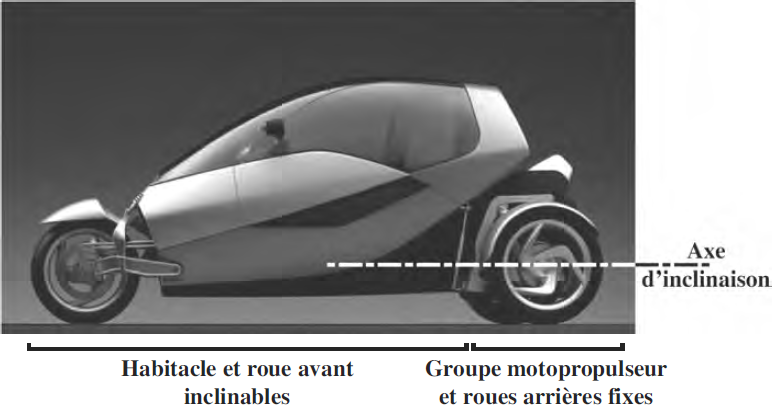
\includegraphics[width=0.75\linewidth]{fig_1_1}

\textit{Présentation du mécanisme d'inclinaison}
\label{fig_1_1}
\end{center}


Pour simplifier l'étude, on ne s'intéresse pas dans un premier temps à la roue avant, ce qui permet de se ramener au système schématisé sur la \autoref{fig_1_2}. On donne les caractéristiques géométriques et cinématiques suivantes :
\begin{itemize}
\item la route \textbf{R} est munie du repère $\rep{g}=\repere{O}{x_g}{y_g}{z_g}$. Le référentiel associé est supposé galiléen;
\item le groupe motopropulseur \textbf{0} est animé d'un mouvement de rotation par rapport au sol dont le centre instantané de rotation est $O$. Le rayon de courbure de la trajectoire du point $C$ dans $\rep{g}$ est $R_C$. Le repère lié à \textbf{0} est $\rep{0}=\repere{O}{x_0}{y_0}{z_0}$ tel que $\vect{z_0}=\vect{z_e}$ et on note $\theta=\angl{x_e}{x_0}=\angl{y_e}{y_0}$. On a donc $OC=R_C\vect{x_0}$. On remarquera bien que $\rep{0}$ est mobile par rapport à $\rep{g}$;
\item l'habitacle \textbf{1} est liée au groupe \textbf{0} par une liaison pivot d'axe $\axe{C}{y_0}$. Le repère lié $\rep{1}=\repere{C}{x_1}{y_1}{z_1}$ est tel que $\vect{y_1}=\vect{y_0}$. On note $\alpha=\angl{x_0}{x_1}=\angl{z_0}{z_1}$ l'angle d'inclinaison du système pendulaire. Le centre de gravité de \textbf{1} est $G$ tel que $\vect{CG}=e\vect{z_1}$ et sa masse est $m$. On note $\inertie{G}{1}$ son opérateur d'inertie en $G$. On considérera que c'est un solide de forme quelconque dont la matrice est donnée dans la base $\mathcal{B}_0$.
\item les roues arrière \textbf{2} et \textbf{3} sont liées au groupe \textbf{0} par des liaisons pivots d'axe $\axe{C}{x_0}$.
\item les contacts entre les roues \textbf{2} et \textbf{3} et la route \textbf{R} ont lieu en $A$ et $B$ définis par 
$\vect{CA}=\dfrac{\ell}{2}\vect{x_0}-r\vect{z_0}$ et $\vect{CB}=-\dfrac{\ell}{2}\vect{x_0}-r\vect{z_0}$ , $r$ désignant 
le rayon des roues et $\ell$ la voie arrière du véhicule. Les contacts sont modélisés par des liaisons sphère-plan de centres
 $A$ et $B$ et de normale $\vect{z_0}$. Le contact dans ces liaisons se fait avec frottement et le coefficient de frottement est
  noté $f$ (on supposera pour simplifier que les coefficients de frottement et d'adhérence sont identiques). Les actions
  mécaniques de la route $R$ sur les roues \textbf{2} et \textbf{3} sont modélisées dans le plan $\angl{x_0}{y_0}$  par des 
  glisseurs en $A$ et $B$ de résultantes 
  $\vectf{R}{2}=T_A\vect{x_0}+N_A\vect{z_0}$  et  $\vectf{R}{3}=T_B\vect{x_0}+N_B\vect{z_0}$.
\end{itemize}

Dans les questions qui suivent, mises à part la liaison entre \textbf{R} et \textbf{2} et celle entre \textbf{R} et \textbf{3}, pour lesquelles le frottement est pris en compte, toutes les liaisons sont considérées parfaites. En outre, on négligera la masse des pièces \textbf{0}, \textbf{2} et \textbf{3} devant celle de l'habitacle \textbf{1}. On note $E=0\cup 1 \cup 2 \cup 3$. L'accélération de la pesanteur est  $\vect{g}=-g\vect{z_0}$.

On se place dans un cas où le rayon de courbure $R_C$ de la trajectoire du point $C$, ainsi que la vitesse $V$ de ce point par rapport au référentiel $\rep{g}$ sont constants. L'angle d'inclinaison $\alpha$  du système pendulaire est lui aussi supposé constant.



\question{Exprimer la vitesse, notée $\vect{V\left(G/\rep{g}\right)}$, du point $G$ dans son mouvement par rapport à $\rep{g}$ en fonction de $V$, $e$, $R_C$ et $\alpha$.}
\ifprof
\begin{corrige}
\end{corrige}
\else
\fi


\question{Exprimer l'accélération, notée $\vect{a\left(G/\rep{g}\right)}$, du point $G$ dans son mouvement par rapport à $\rep{g}$ en fonction de $V$, $e$, $R_C$ et $\alpha$.}
\ifprof
\begin{corrige}
\end{corrige}
\else
\fi

On 

\begin{center}%[H]
\centering
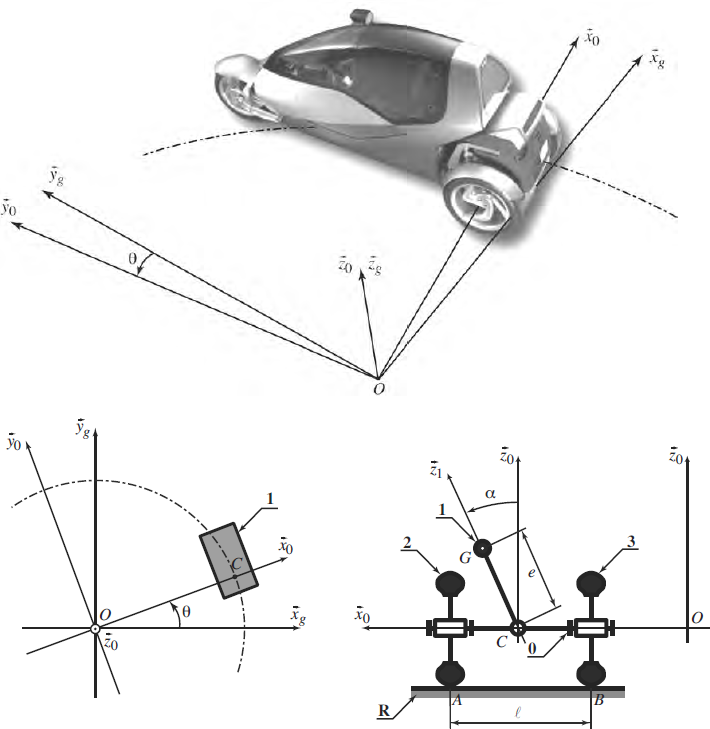
\includegraphics[width=0.75\linewidth]{fig_1_2_all}

\textit{Modélisation simplifiée du Clever en position inclinée}
\label{fig_1_2}
\end{center}
 
 \textbf{On néglige le contact entre la roue avant et le sol.}
 
\question{En rappelant que le rayon $R_c$, la vitesse $V$ et l'angle $\alpha$ sont supposés constants, calculer le moment dynamique en G$,$ noté $\vectmd{G}{E}{\rep{g}}$, de l'ensemble $E$ dans son mouvement par rapport à $\rep{g}$. }
\ifprof
\begin{corrige}
\end{corrige}
\else
\fi

\question{En appliquant le principe fondamental de la dynamique à l'ensemble $E$ dans son mouvement par rapport à $\rep{g}$, écrire les trois équations scalaires qui lient les actions mécaniques de contact entre le sol et les roues $T_A$, $N_A$, $T_B$ et $N_B$ aux données du problème.}
\ifprof
\begin{corrige}
\end{corrige}
\else
\fi

\question{Déduire de ces trois relations l'expression des efforts normaux $N_A$ et $N_B$ en fonction de $m$, $\ell$, $r$, $e$, $g$ et $R_c$, $\alpha$, $V$. Tous les autres paramètres étant fixés, une augmentation de la vitesse $V$ risque-t-elle de susciter un décollement de la roue intérieure ou de la roue extérieure au virage ?}
\ifprof
\begin{corrige}
\end{corrige}
\else
\fi


\question{Déduire de la question précédente la condition de non renversement, écrite sous la forme d'une inéquation, qui lie le rapport $V^2/R_c$ aux paramètres $\ell$, $r$, $e$, $g$ et $\alpha$, $R_c$.}
\ifprof
\begin{corrige}
\end{corrige}
\else
\fi


\question{Exprimer les conditions d'adhérence liant $T_A$, $T_B$, $N_A$, $N_B$ et $f$. En utilisant les équations qui avaient été montrées précédemment et en appliquant le principe fondamental de la dynamique, en déduire la condition d'adhérence, écrite sous la forme d'une inéquation, qui lie le rapport $\dfrac{V^2}{R_c}$ aux paramètres $e$, $f$, $g$ et $\alpha$, $R_c$.}
\ifprof
\begin{corrige}
\end{corrige}
\else
\fi
 
 
 
\subsection{Cas d'un véhicule sans architecture pendulaire}
 Afin de montrer l'intérêt de l'architecture pendulaire comme solution technique à la fonction de service FS3 «~S'insérer facilement dans la circulation~», on imagine maintenant que le véhicule Clever n'en est pas équipé, ce qui se traduit par la condition $\alpha = 0$.
 
 
\question{Réécrire les conditions d'adhérence et de non renversement dans ce cas particulier. }
\ifprof
\begin{corrige}
\end{corrige}
\else
\fi

\vspace{.5cm}
 
 On se propose d'étudier la configuration suivante :
 \begin{itemize}
 \item rayon d'une roue, $r = \SI{30}{cm}$, position du centre de gravité, $e = \SI{50}{cm}$;
 \item accélération de la pesanteur, $g = \SI{9,81}{m.s^{-2}}$ coefficient d'adhérence pneu-route, $f = 0,8$.
\end{itemize}


\question{Calculer la valeur de la voie arrière du véhicule (largeur $\ell$ entre les roues arrières) en dessous de laquelle le phénomène limitant la vitesse à laquelle on peut prendre un virage est le risque de renversement et non celui de dérapage. En déduire quel est le phénomène limitant dans le cas d'une voiture traditionnelle (voie de l'ordre de \SI{1,5}{m}) et dans le cas d'un véhicule étroit comme le Clever (voie égale à \SI{0,9}{m}) ?}
\ifprof
\begin{corrige}
\end{corrige}
\else
\fi



\question{Calculer la valeur de la vitesse maximale $V$ à laquelle il est possible de prendre un virage de rayon de courbure $R_c = \SI{20}{m}$ avec un véhicule étroit de voie $\ell = \SI{0,9}{m}$ si celui-ci n'est pas inclinable. On exprimera cette vitesse en km/h. Celle-ci est-elle compatible avec la norme qui prescrit de pouvoir rouler à $\SI{55}{km.h^{-1}}$ dans un virage de rayon de courbure \SI{20}{m} ?}
\ifprof
\begin{corrige}
\end{corrige}
\else
\fi


\subsection{Cas d'un véhicule à architecture pendulaire}

On considère maintenant l'architecture pendulaire. L'angle a peut varier dans la plage $[- 45\degres, 45\degres]$.

\question{Commenter le signe de l'angle $\alpha$ pour contribuer au non renversement du Clever dans la configuration de la 
\autoref{fig_1_2} (virage à gauche). Le véhicule doit-il s'incliner vers l'intérieur ou vers l'extérieur de la trajectoire (comme c'est le cas sur la \autoref{fig_1_2} en bas à droite) ? }
\ifprof
\begin{corrige}
\end{corrige}
\else
\fi

Le graphique de la \autoref{fig_1_3}, représente, en fonction de l'angle d'inclinaison $\alpha$ et dans la configuration précédente (même géométrie et rayon de courbure $R_c = \SI{20}{m}$), l'évolution de vitesse maximale $V$ en dessous de laquelle il n'y a pas renversement.



\question{En utilisant la \autoref{fig_1_3}, déterminer l'angle d'inclinaison a qu'il faut imposer à l'habitacle pour respecter la norme. }
\ifprof
\begin{corrige}
\end{corrige}
\else
\fi

\begin{center}%[H]
\centering
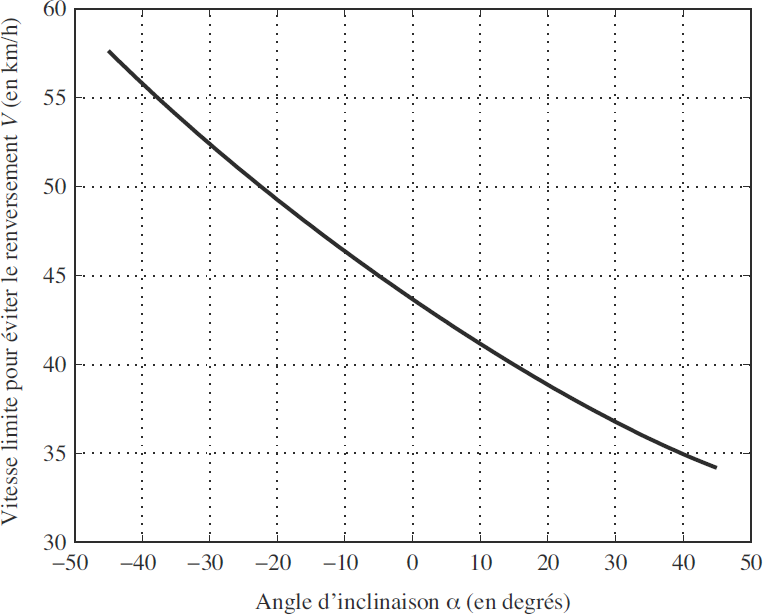
\includegraphics[width=0.65\linewidth]{fig_1_3}

\textit{Représentation graphique de la condition de non renversement}
\label{fig_1_3}
\end{center}


\ifprof
%\end{multicols}%
\else
\end{multicols}%
\fi

